\chapter{Evaluation}

This chapter covers the evaluation of the final product, the process model and what the team learned in this course.

\section{Problems and Difficulties}
	The first problem the group encountered, was to not use incompatible licenses. This was quite hard because much is licensed as GPL 1 or 2 and are not compatible with Apache 2. \\

	The second problem was the decision to write the protocol or use a middleware on a computer.

	The last problem was to get the protocol to work.

\subsection{Protocol}
There were several difficulties related to programming the Arduino. There were few existing solutions for programming it in general, and none for Android or Java. The official implementation was available in C, but in the incompatible GPL license.\\

The existence of certain programs written in Java with the purpose of programming Arduinos,
led the group into assuming one of these could be utilized, as the license was compatible. When the time came to make use of it, it was discovered to internally use AVRDUDE as well - an embedded version was available for several platforms.\\

This realization came somewhat late in the process, see Iteration 4 in the appendix on page \pageref{Iteration4}. Following this and the emergency meeting with the customer, it was decided to implement the protocol for programming Arduinos. Unfortunately, the documentation for these were a bit confusing; the most detailed and professional protocol document turned out to describe version 2 of the protocol, which was incompatible with the bootloader installed on the Arduino by default (Optiboot v4.4 on Arduino Uno). This was also the version that was partially implemented before the protocol differences and lack of backwards compatibility was discovered.\\

Changing the bootloader to utilize version 2 of the protocol could not be done due to it being licensed under GPL. Some attempts were made at finding compiled bootloaders for the Uno, but did not bear fruit. Attempts at compiling bootloaders using version 2 for the chip failed due to unresolved dependencies in the bootloader projects discovered. # Should have references to those projects here!\\

The solution, then, was to implement version 2 of the protocol, and write off most of the protocol work as waste (a bit less than a week); some of it could be reused despite the protocols being radically different, however. The second version of the protocol has a standardized message format with checksums and static tokens inside the messages to aid in error discovery; this would have been beneficial for communicating over Bluetooth.\\



			- Used more time than expected\\
			- Change from STK500v2 to STK500v1\\
			- Had major impact on the project\\
			- Not enough research on the protocol in the beginning of the project\\

\section{Interaction with the customer}
	The communication with the customer was great. A regular meeting was held every Friday, and the customer had an insight to the projects repositories, so the customer always knew what was going on.

\section{Usage of workhours}
	The group decided from the beginning that every member should work approximately 20 hours every week.
	In Table ~\ref{table:workhours} it is listed the total work hours for the group on every iteration.

	\begin{table}[H]
	\caption{Iterations and time spent}
	\centering
	\label{table:workhours}
	\begin{tabular}{|l|l|}
		\hline
			{\bf Iteration} & {\bf Hours}\\
		\hline
			Iteration 1 (Week 6-7) & 186 hours\\
		\hline
			Iteration 2 (Week 8-9) & 257 hours\\
		\hline
			Iteration 3 (Week 10-11) & 233 hours\\
		\hline
			Iteration 4 (Week 12-13) & 129 hours\\
		\hline
			Iteration 5 (Week 14-15) & 195 hours\\
		\hline
			Iteration 6 (Week 16-17) & 220 hours\\
		\hline
			Iteration 7 (Week 18-19) & 263 hours\\
		\hline
	\end{tabular}
	\end{table}

	An associated chart diagram of the workhours are shown in Figure ~\ref{fig:workhours}

	\begin{figure}[H]
	\centering
	\captionof{figure}{Workhours in each iteration}
	\label{fig:workhours}
	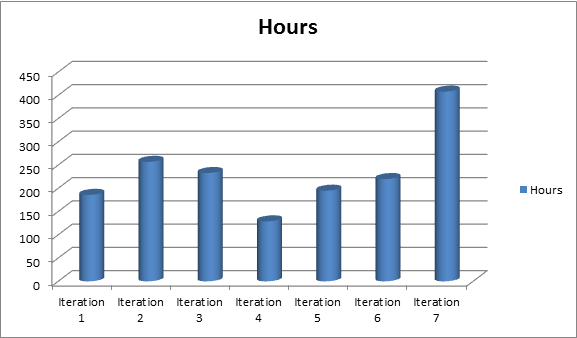
\includegraphics[scale=0.8]{images/workhours_chart2.png}
	\end{figure}

	\section{Process}
	The overall process has been going well. The group have learned to document issues and tasks on the way. This made the process flow steady forward and made it clear and organized. Every member always knew what to do when he or her checked the issue list on Git.

	The communication in the group was also good when the group worked together almost every day and had a group meeting every week. The group could also contact each other via Skype, phone and email.

	\section{The System}
	The $\mu$C Software Store application is almost ready to use. A few changes is still needed to be implemented before it can enter the market. \\

	- Focused too much on the application\\
	- Focused too little on the protocol

		\subsection{Requirements met}
			- GUI\\
			- Bluetooth connection\\
			- QR-code and SerialInput\\
			- Filter application by compatibility\\
			- Retain a reliable connection to the connected device\\
			- Remember the device from last time and try to reconnect\\

		\subsection{Requirement not met}
			- Sync Adapter\\
			- External database\\
			-

	\section{Conclusion}
    Placeholder text
